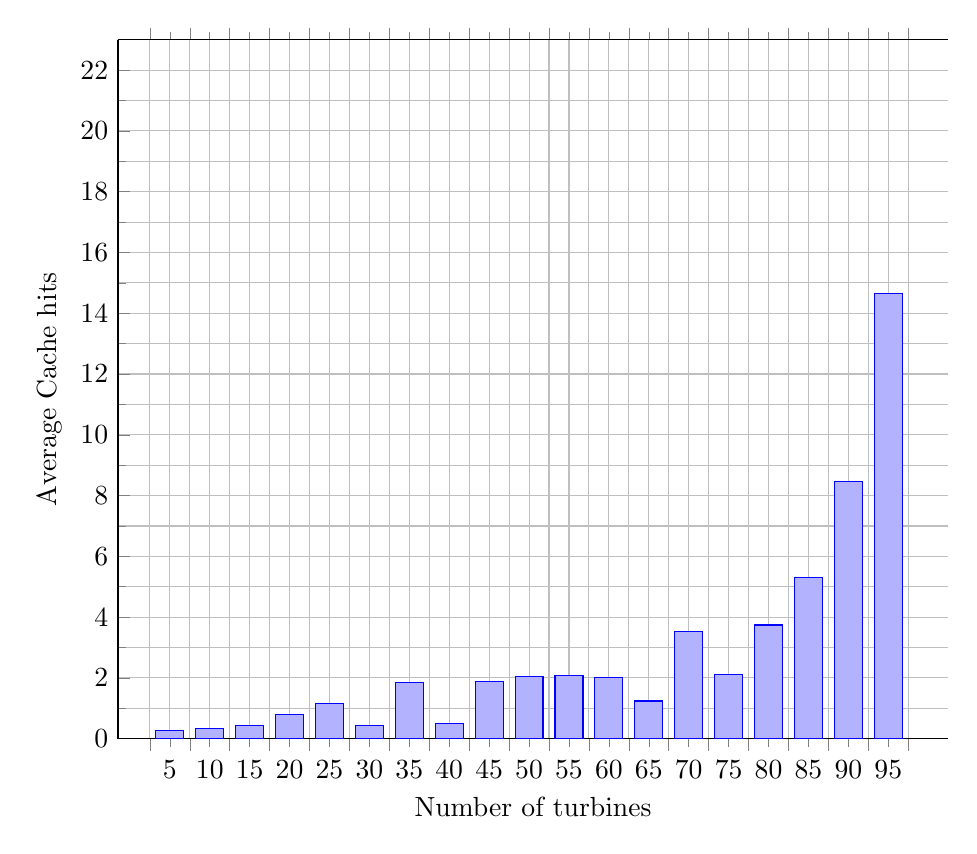
\begin{tikzpicture}
\begin{axis}
[
width=\resultsPlotWidthScale\textwidth,
axis y line*=left,
xlabel=Number of turbines,
ymin = 0, ymax = 23,
xmin = 1, xmax = 105,
ylabel=Average Cache hits,
%xtick={1, 2, 3, 4, 5, 6, 7, 8, 9, 10, 11, 12, 13, 14, 15, 16, 17, 18, 19, 20},
%xticklabels={5, 10, 15, 20, 25, 30, 35, 40, 45, 50, 55, 60, 65, 70, 75, 80, 85, 90, 95, 100},
%boxplot/draw direction=y,
ybar interval=0.7,
grid=both,
minor tick num=1
]
%\buildBoxPlot[black]{0}{0}{0}{0}{0}
%\buildBoxPlot[black]{0}{0}{0}{0}{0}
%\buildBoxPlot[black]{0}{0}{0}{0}{0}
%\buildBoxPlot[black]{0}{0}{0}{0}{0}
%\buildBoxPlot[black]{0}{0}{0}{0}{0}
%\buildBoxPlot[black]{0}{0}{0}{0}{0}
%\buildBoxPlot[black]{0}{0}{0}{0}{0}
%\buildBoxPlot[black]{0}{0}{0}{0}{0}
%\buildBoxPlot[black]{0}{0}{0}{0}{0}
%\buildBoxPlot[black]{0}{0}{0}{0}{0}
%\buildBoxPlot[black]{0}{0}{0}{0}{0}
%\buildBoxPlot[black]{0}{0}{0}{0}{0}
%\buildBoxPlot[black]{0}{0}{0}{0}{0}
%\buildBoxPlot[black]{0}{0}{0}{0}{0}
%\buildBoxPlot[black]{0}{0}{0}{0}{0}
%\buildBoxPlot[black]{0}{0}{0}{0}{0}
%\buildBoxPlot[black]{0}{0}{0}{0}{0}
%\buildBoxPlot[black]{0}{0}{0}{0}{0}
%\buildBoxPlot[black]{0}{0}{0}{0}{0}
%\buildBoxPlot[black]{0}{0}{0}{0}{0}
\addplot coordinates {
	(5 ,0.2591015249347438)
	(10 ,0.3423283799799435)
	(15 ,0.4286200856364344)
	(20 ,0.7913519050319182)
	(25 ,1.171919068056407)
	(30 ,0.4440826120490188)
	(35 ,1.8595523144717856)
	(40 ,0.506366007056297)
	(45 ,1.8951768000539848)
	(50 ,2.037951753081981)
	(55 ,2.0728170589196186)
	(60 ,2.0275369832294468)
	(65 ,1.2416290071090674)
	(70 ,3.5220372523313626)
	(75 ,2.115832267020478)
	(80 ,3.7417427229878832)
	(85 ,5.311682134712245)
	(90 ,8.473847137142263)
	(95 ,14.663734246038112)
	(100 ,22.06932793366117)
};

%	\addplot[
%	blue,
%	domain=5:80,
%	samples=5,
%	]
%	{(x*0.02964) + 0.1108};

%     General model:
%     f(x) = exp(x*a)*b +c
%     Coefficients (with 95% confidence bounds):
%     a =     0.09968  (0.08592, 0.1134)
%     b =   0.0009945  (-0.0003517, 0.002341)
%     c =       1.047  (0.6037, 1.49)

%	\addplot[
%	black,
%	domain=5:100,
%	samples=201,
%	]
%	{exp(x*0.09968)*0.0009945+1.047};

\end{axis}
\end{tikzpicture}